\documentclass[lang=cn, 10pt, titlestyle=hang]{elegantbook}
\usepackage{graphicx}
\usepackage{subfigure}
\usepackage{pgfplots}
\pgfplotsset{compat=1.18}
\renewcommand{\theequation}{\Roman{equation}}

\title{九年级数学讲义(人教版)}


\begin{document}

\tableofcontents

\chapter{一元二次方程}



\begin{introduction}[本章学习目标]

\item 将一元二次方程整理为一般形式
\item 判定一元二次方程
\item 熟练掌握配方法
\item 使用配方法求最值
\item 用不同方式解一元二次方程

\end{introduction}

经过本章的学习,你至少需要掌握以上的内容,在完成学习后你可以根据习题的情况,对照上面的学习目标,检验自己的学习成果.

\section{一元二次方程基本}
\subsection{一元二次方程的定义}


\begin{definition}
  
等号两边都是整式,只含一个未知数,并且未知数的最高次数是2的方程,叫做一元二次方程. 以下是二元一次方程的一般形式:

\begin{equation}
    ax^2 + bx + c = 0 \ (a \neq 0)
    \label{general_formula}
\end{equation}

 
\end{definition}



根据课本的定义,要构成一个一元二次方程必须具有三个条件:
\begin{enumerate}
    \item 是整式方程
    \item 只含有一个未知数
    \item 未知数的最高次数为2
\end{enumerate}
\par
%定义例题
\begin{example}
    下列关于 \( x \) 的方程中,一定是一元二次方程的为({\hspace{3.5em}})。
    \begin{enumerate}[label=\Alph*.]
        \item \( x^2 + 2xy + y^2 = 0 \)
        \item \( x^2 - 2x + 3 = 0 \)
        \item \( x^2 - \frac{1}{x} = 0 \)
        \item \( ax^2 + bx + c = 0 \)
    \end{enumerate}
\end{example}



\begin{solution}
    阅读题目,要我们选出一定是一元二次方程的方程,需要结合一元二次方程的定义来解题,看每个选项是否符合一元二次方程必须具有的三个条件.
    \begin{enumerate}[label=\Alph*.]
        \item 是整式方程,未知数的最高次数为2,但含有两个未知数(\(x,y\)),所以错误.
        \item 是整式方程,只含有一个未知数,未知数的最高次数为2,满足所有条件所以正确.选择B.
        \item 未知数的最高次数为2,之含有一个未知数,但是是分式方程(分母含有未知数),所以错误.
        \item 是整式方程,未知数的最高次数为2,但是a的取值无法确定,当\(a=0\)时,方程中的未知数的最高次数为1,不一定是一元二次方程,因为题目要求“一定是”,所以错误.
    \end{enumerate}
\end{solution}


\begin{definition}
    我们将\eqref{general_formula}中的$ax^2$称为二次项(未知数的次数为2),a是二次项的系数;$bx$称为一次项(未知数的次数为1),$b$是一次项系数;$c$称为常数项.
\end{definition}
\begin{definition}
    $x$的值就是这个一元二次方程的解,也可以称作这个一元二次方程的根.\\
    \begin{remark}
        在做题时,有时会把$x$的值称做方程的解,有时称作方程的根,其实这都是一个意思.
    \end{remark}
\end{definition}





\subsection{一元二次方程一般式转化}

在解题时,我们通常会先将一元二次方程整理为一般形式($
ax^2 + bx + c = 0 \ (a \neq 0)
$),这样做可以减少我们的工作量和出错的概率,便于进行计算.



整理过程分两步:
\begin{enumerate}
    \item 移项、合并
    \item 将二次项的系数化为非负数
\end{enumerate}

\subsection{判定一元二次方程}




经过总结,我们可以得到步骤:



\begin{enumerate}
    \item 整理方程
    \item 判断是否符合条件
\end{enumerate}


\begin{exercise}
    \begin{enumerate}
        \item 下列关于 \( x \) 的方程中,是一元二次方程的为({\hspace{3em}})。
        \begin{enumerate}[label=\Alph*.]
            \item \( x^2 + \frac{1}{x} = 0 \)
            \item \( x^2 - xy = 0 \)
            \item \( x^2 + 2x = 1 \)
            \item \( ax^2 + bx = 0 \) (\( a, b \) 为常数)
        \end{enumerate}
    \end{enumerate}
\end{exercise}

\section{配方}



因为某些学校没有详细讲解有关配方法的内容,所以为了更好的理解后面的章节,本节作为补充给没有学过的同学学习。



\begin{example}
    给\( 4x^2 +1\)配上一个单项式,使之成为完全平方式.
\end{example}



分析题目,首先会想到完全平方式的概念是什么,在八上我们学过“两个数的和(或差)的平方,等于它们的平方和,加上(或减去)它们积的2倍.”即以下公式:
$$
(a\pm b)^2 = a^2+b^2\pm 2ab
$$



课本定义的完全平方是狭义的完全平方式,广义上完全平方是指一个数或代数式可以表示为另一个数或代数式的平方,例如\( 1=1^2,\ 4=2^2,\ \)(这些是数的完全平方)\(x^2+6x+9=(x+3)^2,\ 4x^2-12xy+9y^2=(2x-3y)^2\)等等.



根据新学习的完全平方的概念,我们可以知道这道题有多个答案,在做题时要注意紧扣完全平方的定义,分析多种可能结果,不要漏解.
\begin{solution}
    可以配上
\end{solution}

\section{解一元二次方程}
\subsection{配方法(配方后开方降次)}
前面我们学会了使用配方解决问题,配方不仅可以解决一些简单问题,还可以用来解一元二次方程



降次是指通过数学变形(如因式分解、换元、展开等)将一个高次问题转化为低次问题,从而简化计算或求解过程,在初中常用的降次方法有直接开平方法、因式分解法、展开消元法、换元法、公式法,在后面会总结这几种方法并给出例子.



可以将方程式配方,再将两边同时开方使方程(将一元二次方程问题转化为两个一元一次方程问题)

\subsection{公式法}

\subsection{因式分解法}

\chapter{二次函数}

\chapter{旋转}

\section{旋转基本}

\subsection{旋转的性质}

我们把一个平面图形绕着平面内某一点\(O \)转动一个角度,叫做图形的旋转,点\(O \)叫做旋转中心,转动的角叫做旋转角 . 如果图形上的点\(P \)经过旋转变为点\(P' \),那么这两个点叫做这个旋转的对应点.

\begin{example}
    如下图,在\(Rt\triangle ABC \)中,\(\angle ABC = 90^\circ \),\(AB=BC=\sqrt{2}\),将\(\triangle ABC\)绕点\(C\)逆时针旋转\(60^\circ\),得到\(\triangle MNC\),连接\(BM\),则\(BM\)的长是 \underline{\hspace{3em}}
    
\begin{figure}[h]
    \raggedright
    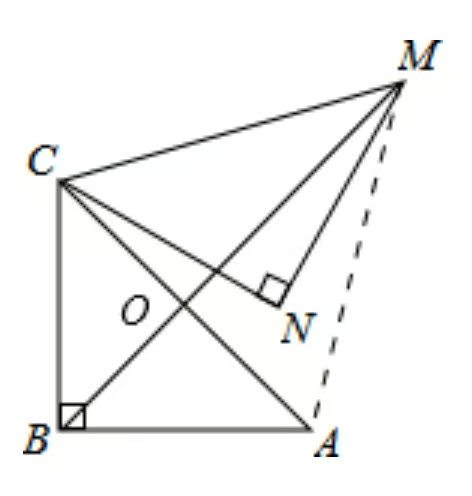
\includegraphics[width=0.25\linewidth]{figure/example_rotation1.jpg}
    
    \label{fig:enter-label}
\end{figure}
    
\end{example}



\chapter{圆}

\chapter{概率初步}

\chapter{反比例函数}

\chapter{相似}

\chapter{锐角三角函数}

\chapter{投影与视图}

\end{document}
